\documentclass[12pt]{article}
\usepackage[top=1in,bottom=1in,left=1in,right=1in]{geometry}
\usepackage{graphicx}

\newcommand{\PstarB}{\mathcal{P}^*_B}
\newcommand{\E}{E}
\newcommand{\sigmacom}{\sigma}
\newcommand{\cmax}{1-(P^*)^{\frac1{k-1}}}
\newcommand{\PZ}{\mbox{PZ}}
\begin{document}


  % Common variance (known and unknown).

  \begin{figure}[tb]
    \center
    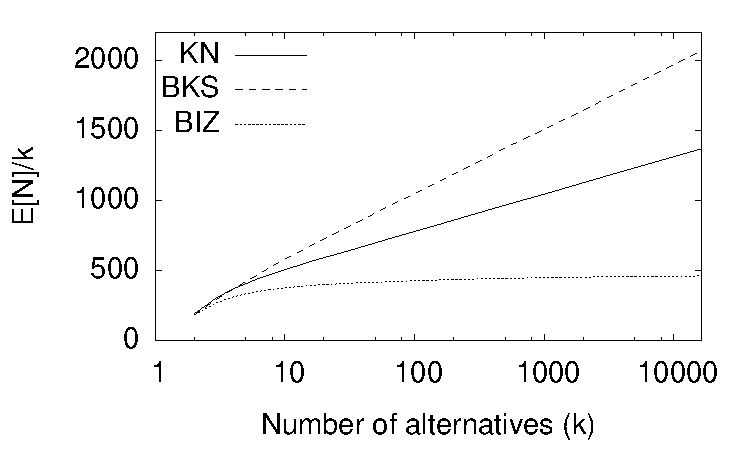
\includegraphics[width=2.9in]{pdf/FINAL-SC-Nk} 
    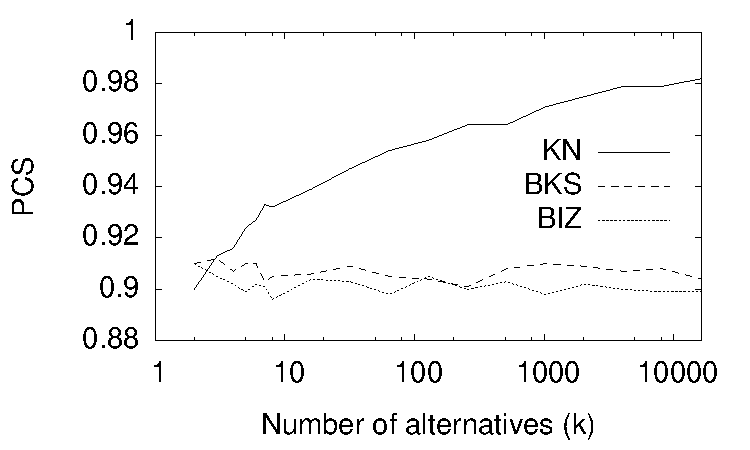
\includegraphics[width=2.9in]{pdf/FINAL-SC-PCS}
    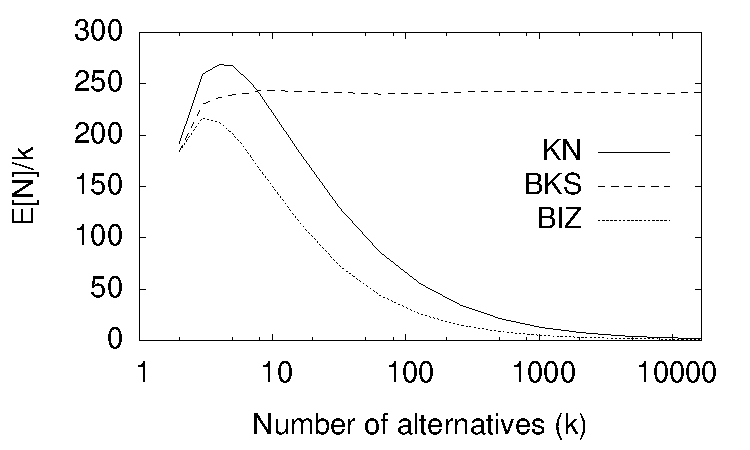
\includegraphics[width=2.9in]{pdf/FINAL-MDM-Nk} 
    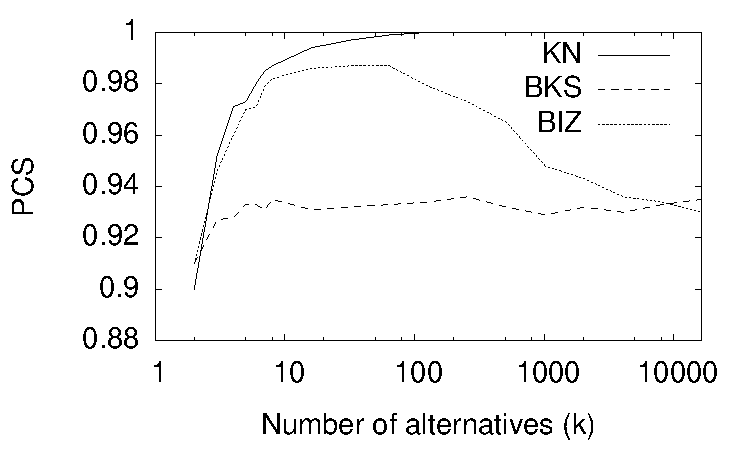
\includegraphics[width=2.9in]{pdf/FINAL-MDM-PCS}
    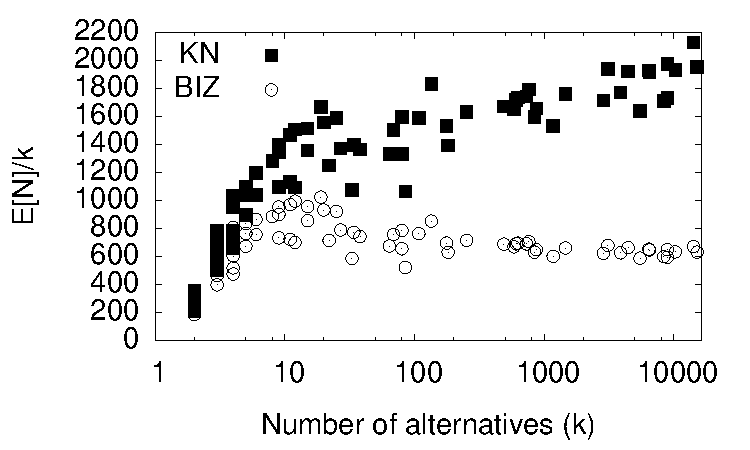
\includegraphics[width=2.9in]{pdf/FINAL-RPI-Nk} 
    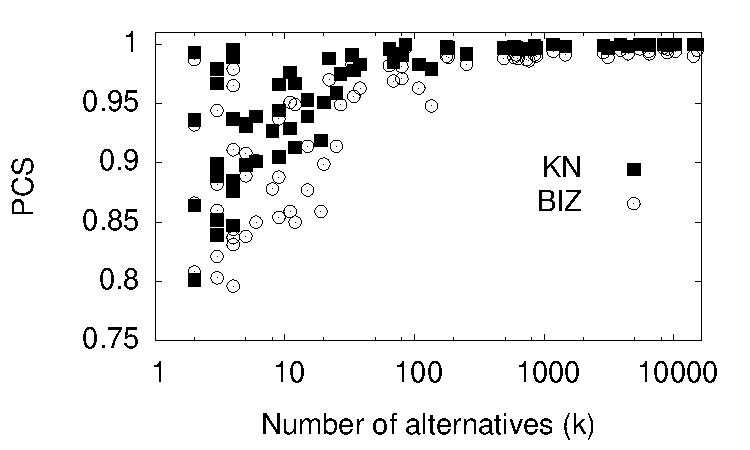
\includegraphics[width=2.9in]{pdf/FINAL-RPI-PCS}

    \caption{Common known variance.  
    First row: SC;
    Second row: MDM;
    Third row: RPI}

  \end{figure}

  \begin{figure}[tb]
    \center
    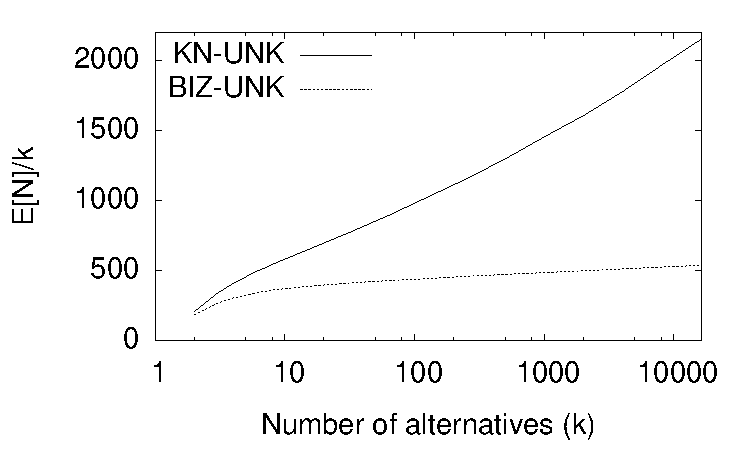
\includegraphics[width=2.9in]{pdf/FINAL-UNK-SC-Nk} 
    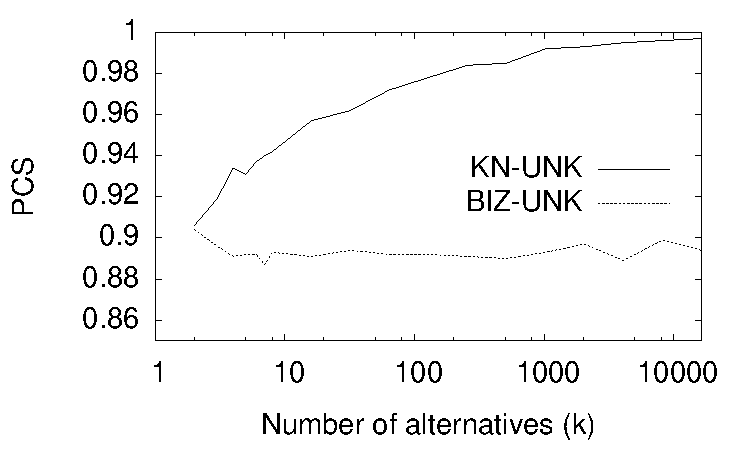
\includegraphics[width=2.9in]{pdf/FINAL-UNK-SC-PCS}
    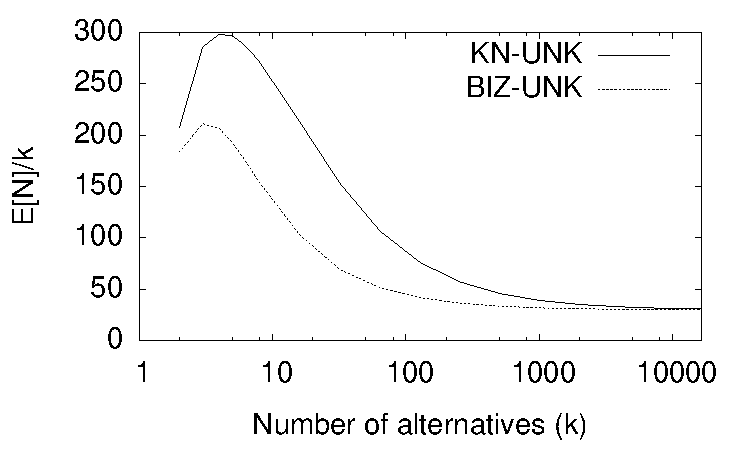
\includegraphics[width=2.9in]{pdf/FINAL-UNK-MDM-Nk} 
    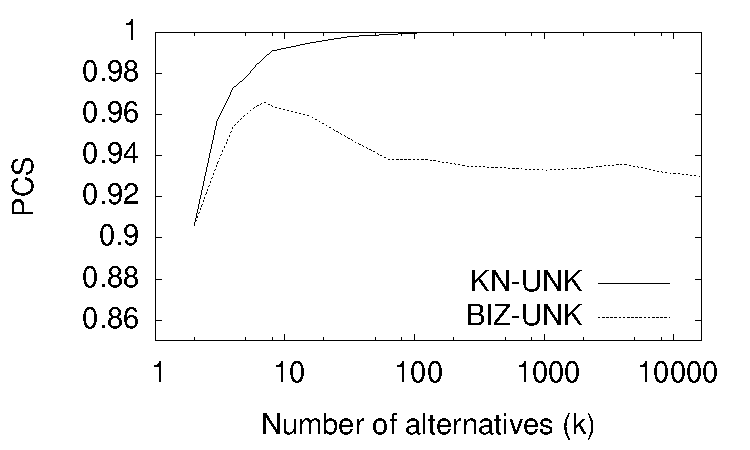
\includegraphics[width=2.9in]{pdf/FINAL-UNK-MDM-PCS}
    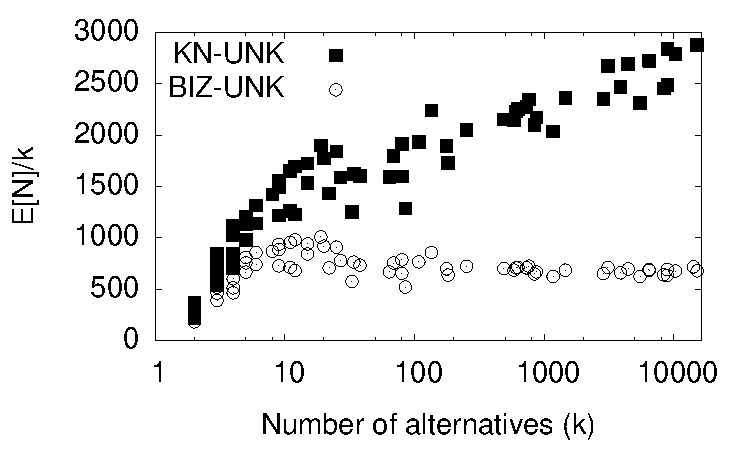
\includegraphics[width=2.9in]{pdf/FINAL-UNK-RPI-Nk} 
    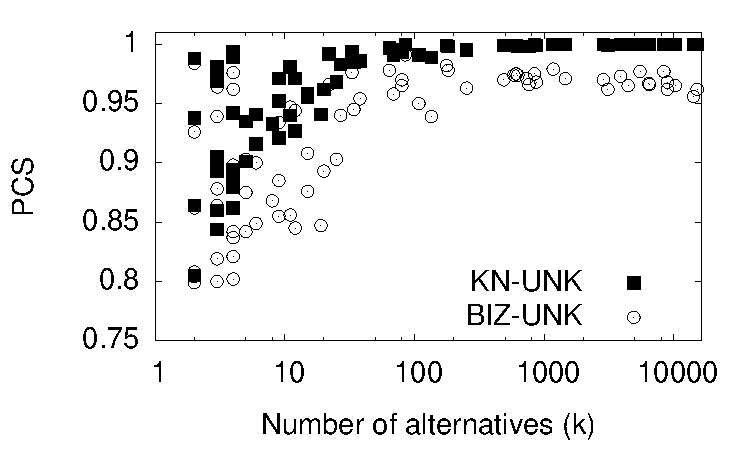
\includegraphics[width=2.9in]{pdf/FINAL-UNK-RPI-PCS}

    \caption{Common unknown variance.  
    First row: SC;
    Second row: MDM;
    Third row: RPI}
  \end{figure}

  % Heterogeneous known variance
 
  \begin{figure}[tb]
    \center
    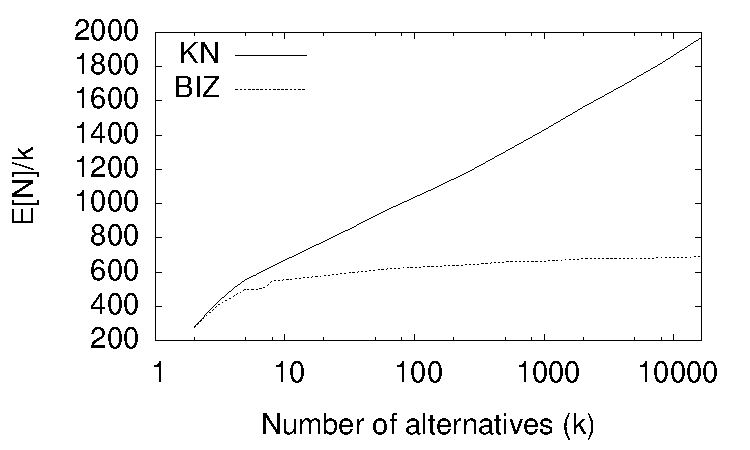
\includegraphics[width=2.9in]{pdf/FINAL-SCINCA-Nk} 
    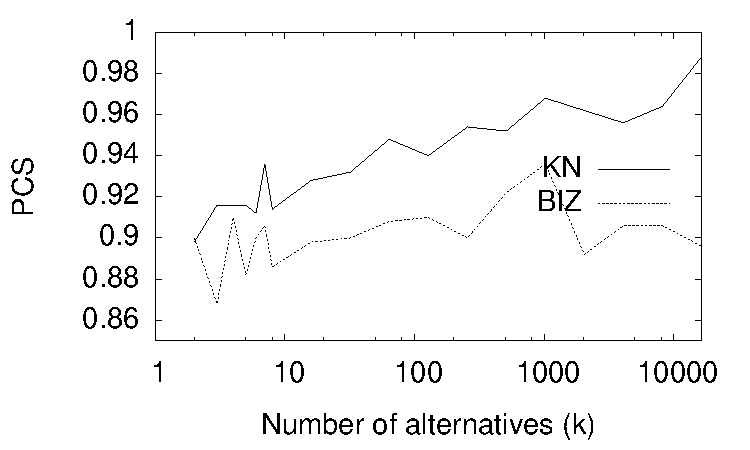
\includegraphics[width=2.9in]{pdf/FINAL-SCINCA-PCS}
    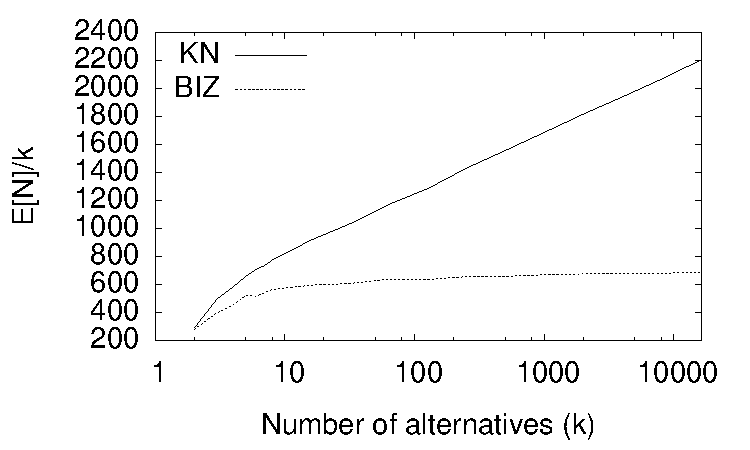
\includegraphics[width=2.9in]{pdf/FINAL-SCDECA-Nk} 
    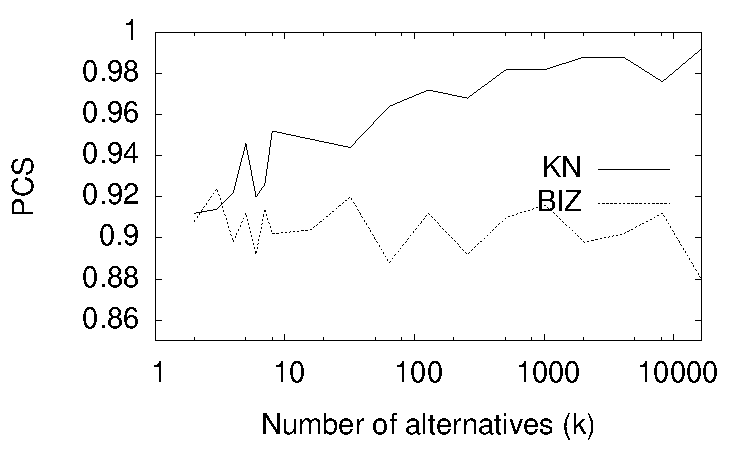
\includegraphics[width=2.9in]{pdf/FINAL-SCDECA-PCS}
    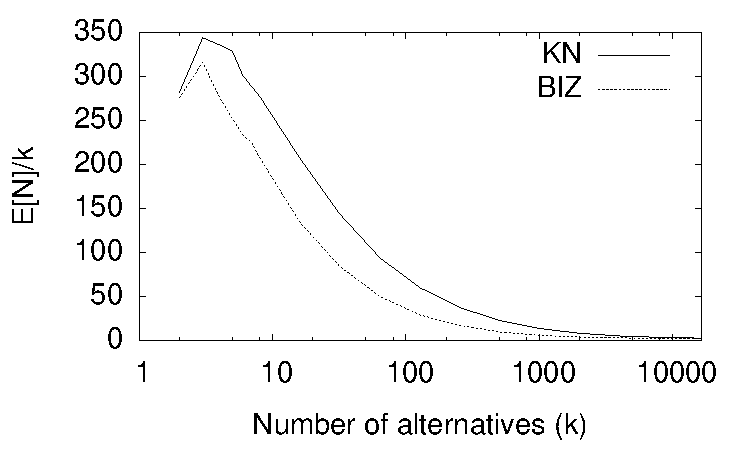
\includegraphics[width=2.9in]{pdf/FINAL-MDMINCA-Nk} 
    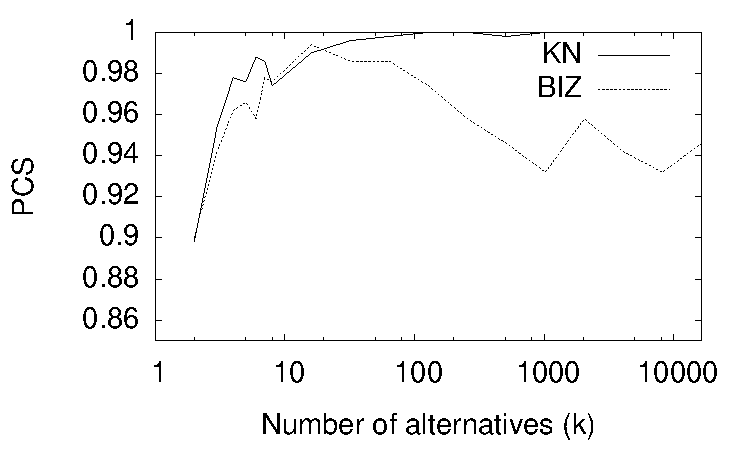
\includegraphics[width=2.9in]{pdf/FINAL-MDMINCA-PCS}
    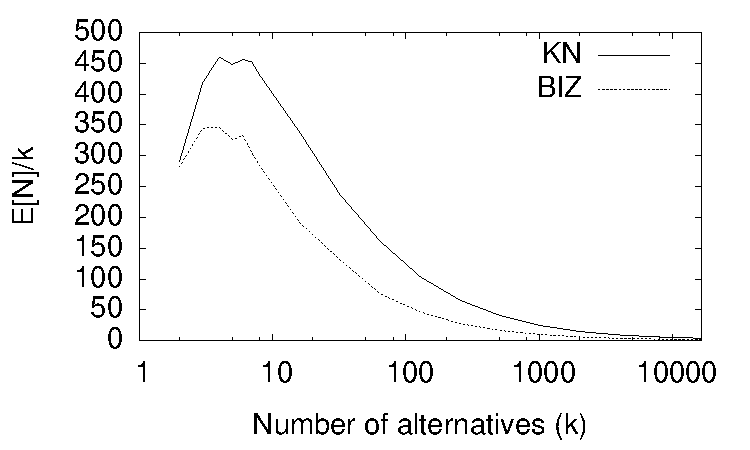
\includegraphics[width=2.9in]{pdf/FINAL-MDMDECA-Nk} 
    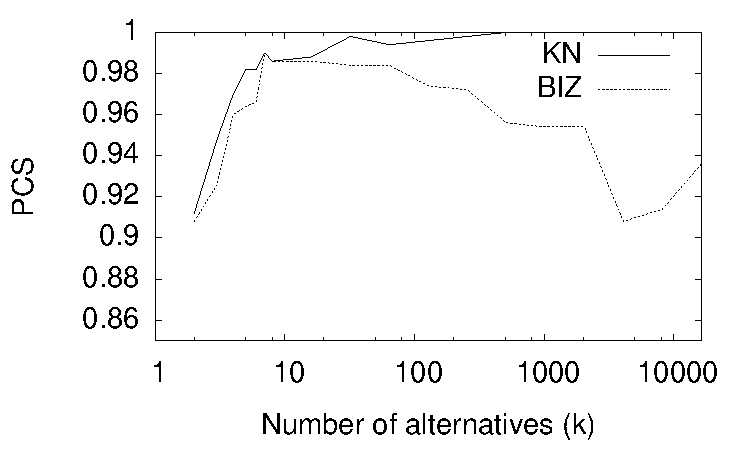
\includegraphics[width=2.9in]{pdf/FINAL-MDMDECA-PCS}
    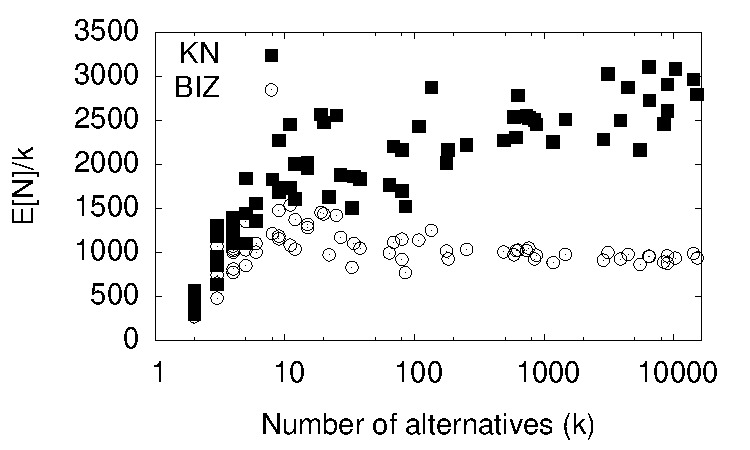
\includegraphics[width=2.9in]{pdf/FINAL-RPIHETA-Nk} 
    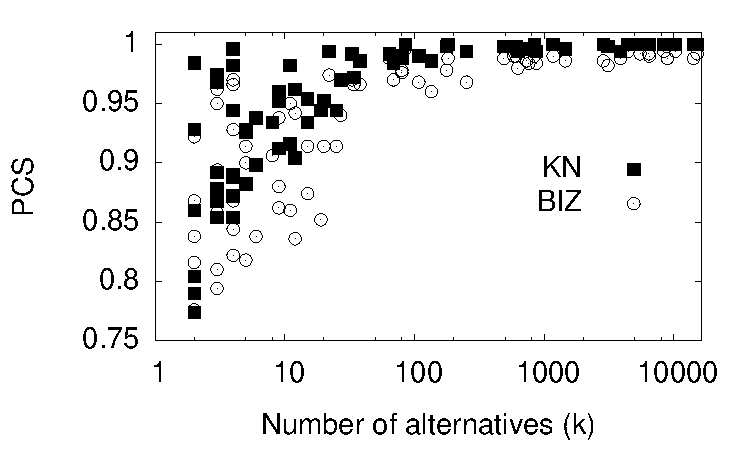
\includegraphics[width=2.9in]{pdf/FINAL-RPIHETA-PCS}

    \caption{Heterogeneous known variance, factor of 2 between largest and smallest variances. 
    Row 1: SCINCA;
    Row 2: SCDECA;
    Row 3: MDMINCA;
    Row 4: MDMDECA;
    Row 5: RPIHETA.
    }
  \end{figure}

  \begin{figure}[tb]
    \center
    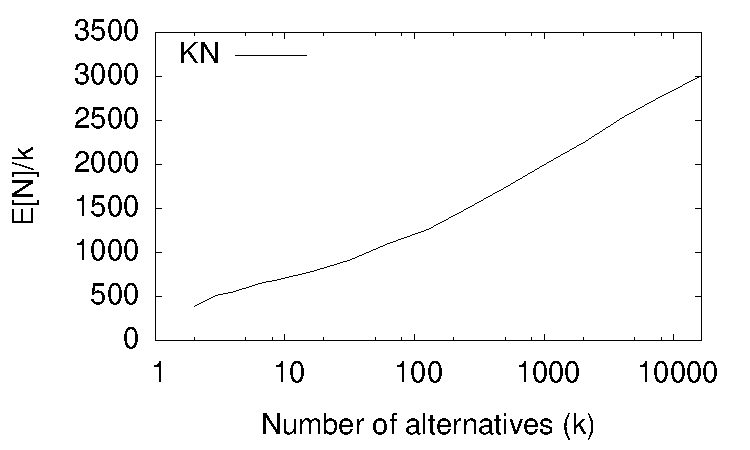
\includegraphics[width=2.9in]{pdf/FINAL-SCINC-Nk} 
    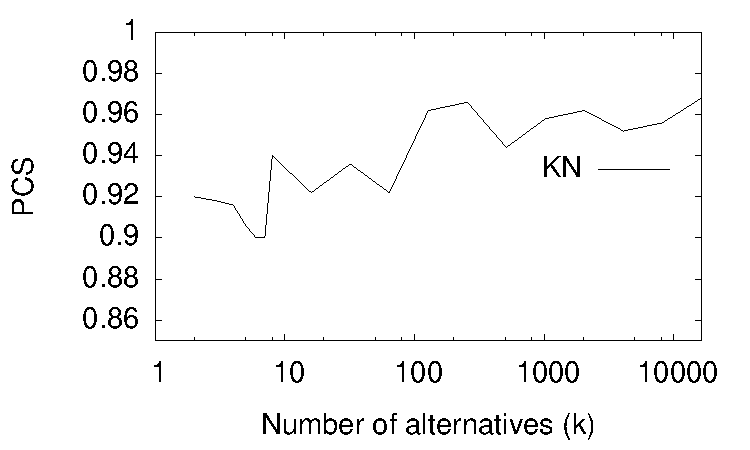
\includegraphics[width=2.9in]{pdf/FINAL-SCINC-PCS}
    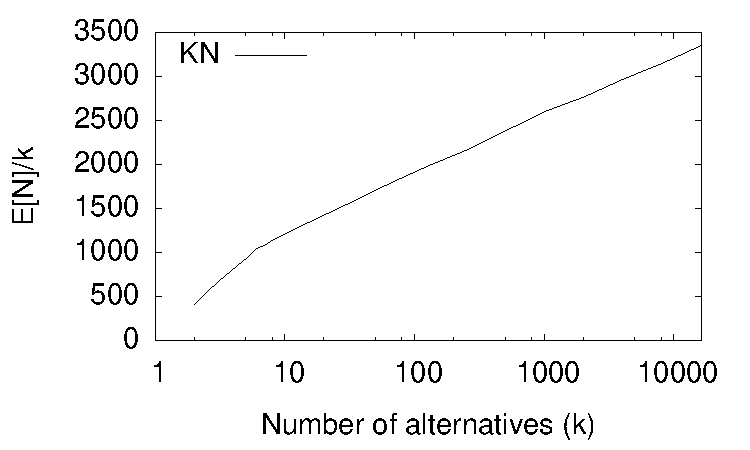
\includegraphics[width=2.9in]{pdf/FINAL-SCDEC-Nk} 
    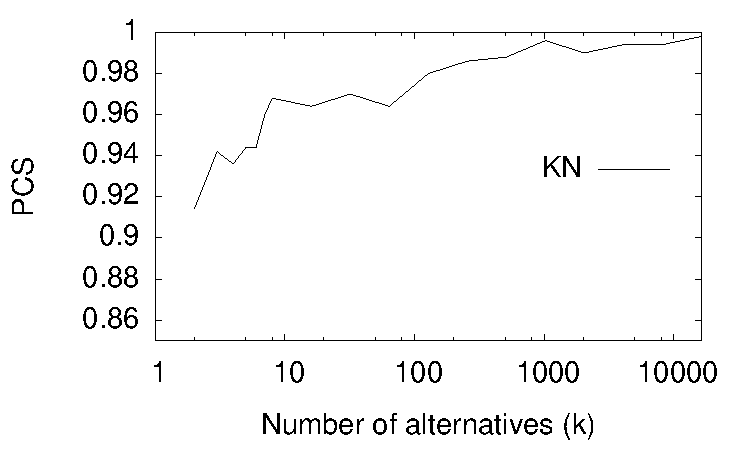
\includegraphics[width=2.9in]{pdf/FINAL-SCDEC-PCS}
    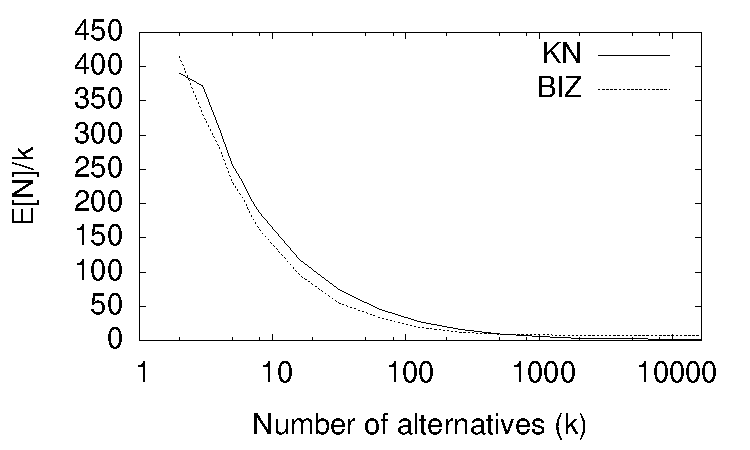
\includegraphics[width=2.9in]{pdf/FINAL-MDMINC-Nk} 
    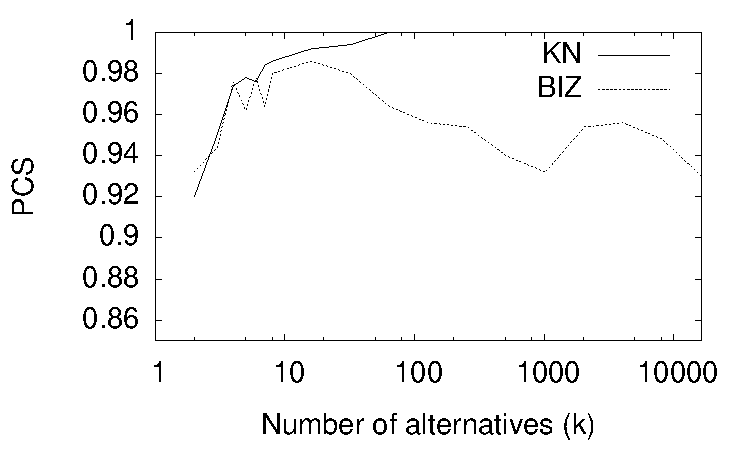
\includegraphics[width=2.9in]{pdf/FINAL-MDMINC-PCS}
    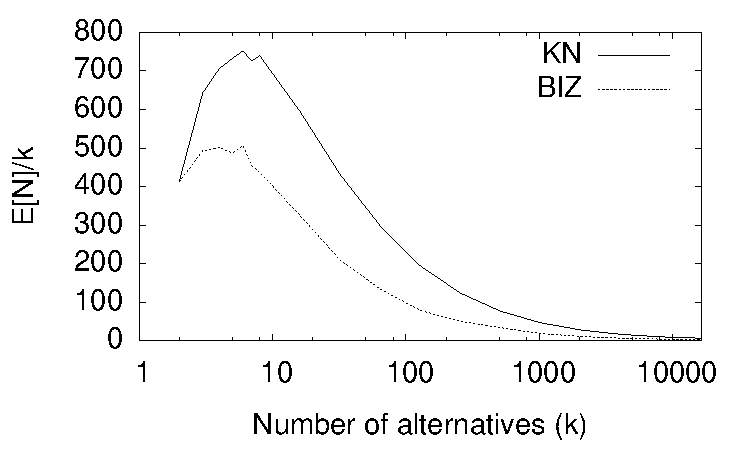
\includegraphics[width=2.9in]{pdf/FINAL-MDMDEC-Nk} 
    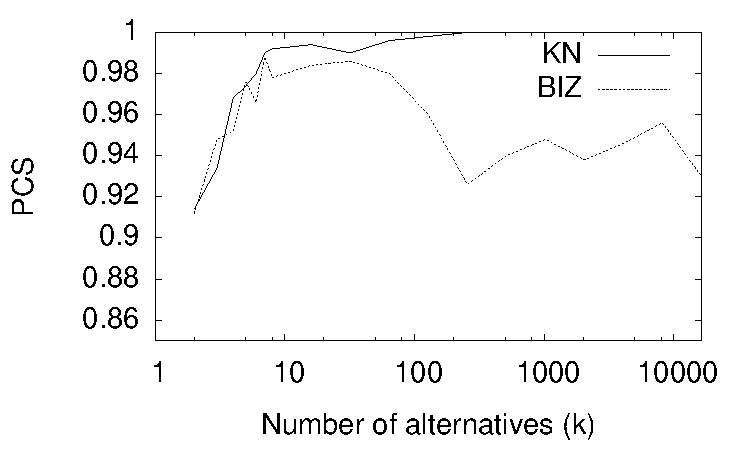
\includegraphics[width=2.9in]{pdf/FINAL-MDMDEC-PCS}
    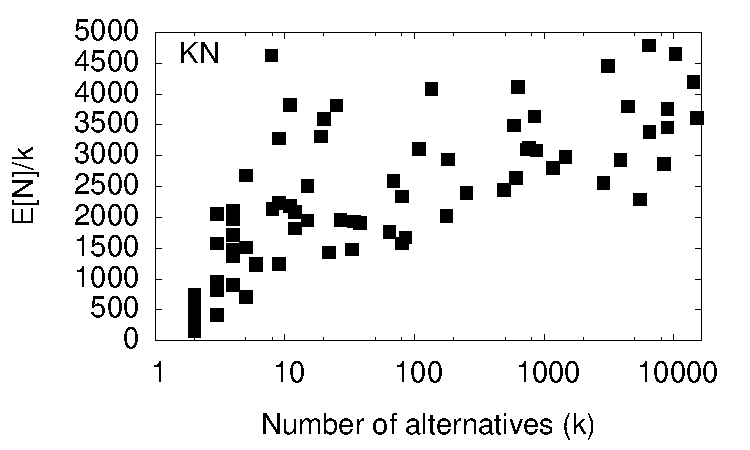
\includegraphics[width=2.9in]{pdf/FINAL-RPIHET-Nk} 
    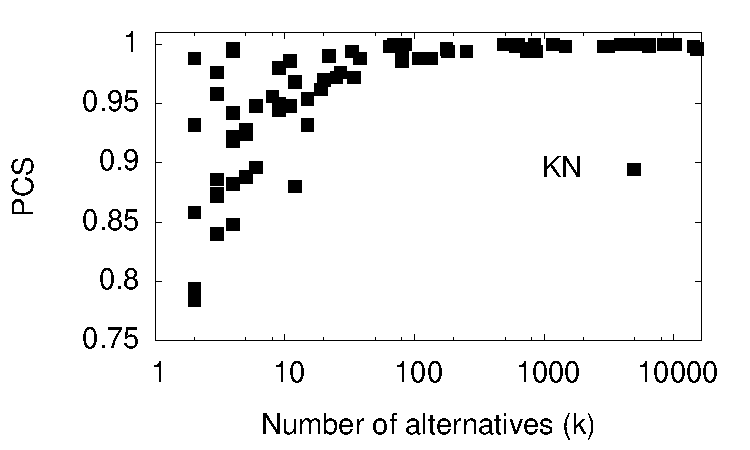
\includegraphics[width=2.9in]{pdf/FINAL-RPIHET-PCS}

    \caption{Heterogeneous known variance, factor of 16 between largest and smallest variances. 
    Row 1: SCINC;
    Row 2: SCDEC;
    Row 3: MDMINC;
    Row 4: MDMDEC;
    Row 5: RPIHET.
    }
  \end{figure}

  % Heterogeneous unknown variance

  \begin{figure}[tb]
    \center
    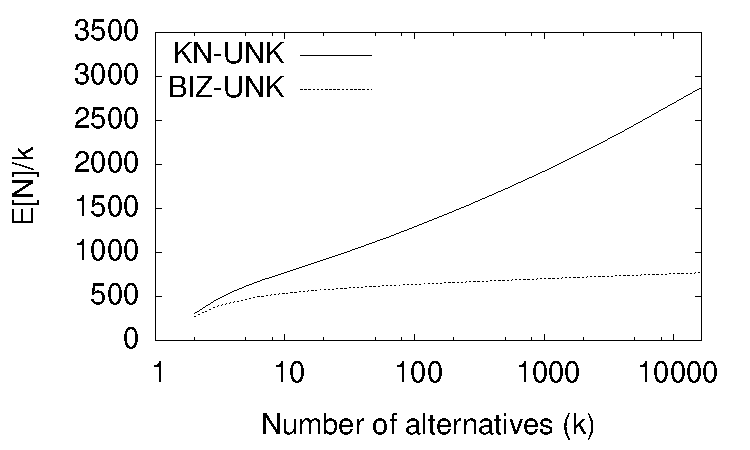
\includegraphics[width=2.9in]{pdf/FINAL-UNK-SCINCA-Nk} 
    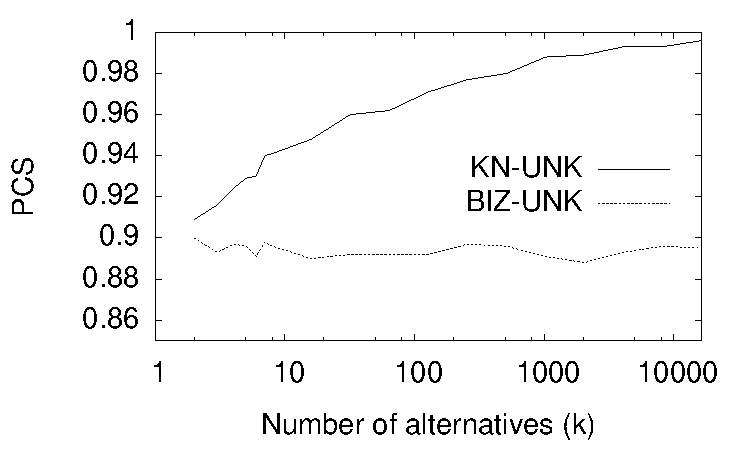
\includegraphics[width=2.9in]{pdf/FINAL-UNK-SCINCA-PCS}
    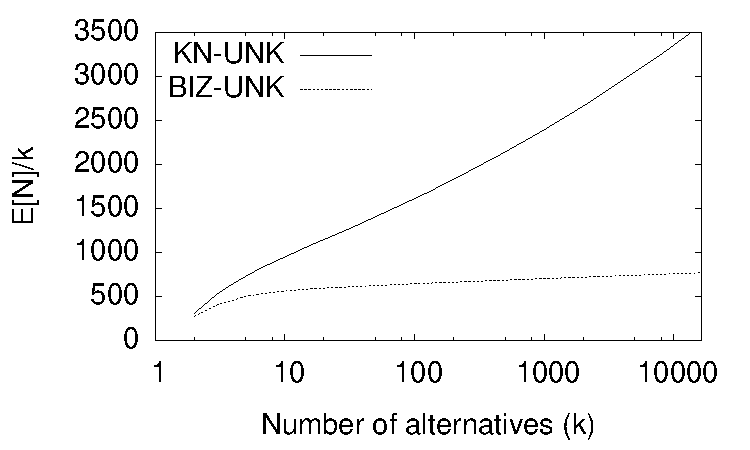
\includegraphics[width=2.9in]{pdf/FINAL-UNK-SCDECA-Nk} 
    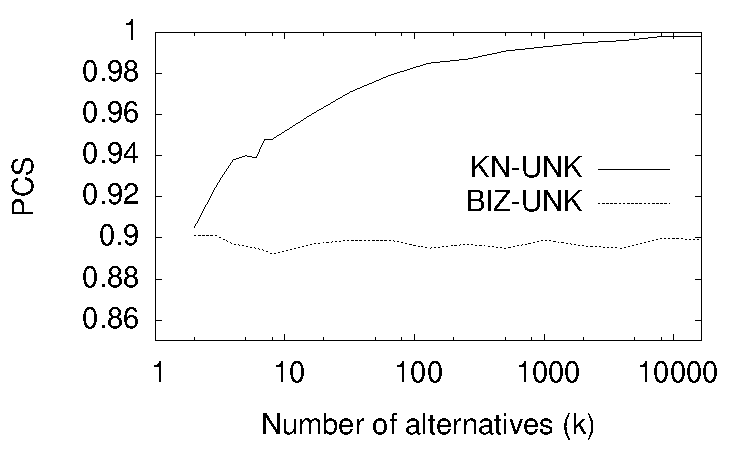
\includegraphics[width=2.9in]{pdf/FINAL-UNK-SCDECA-PCS}
    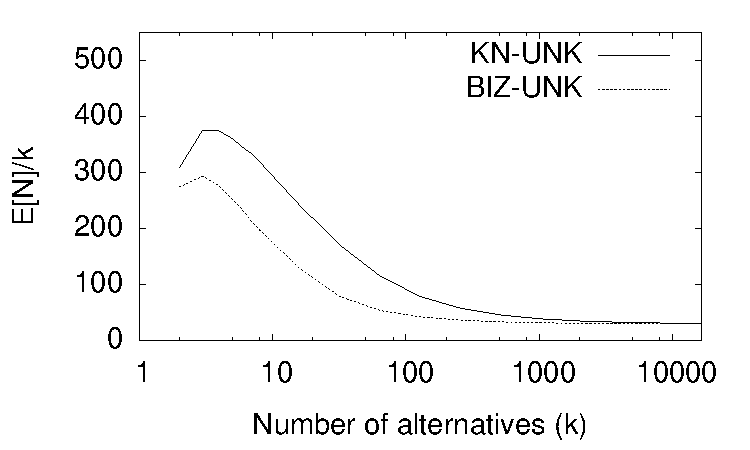
\includegraphics[width=2.9in]{pdf/FINAL-UNK-MDMINCA-Nk} 
    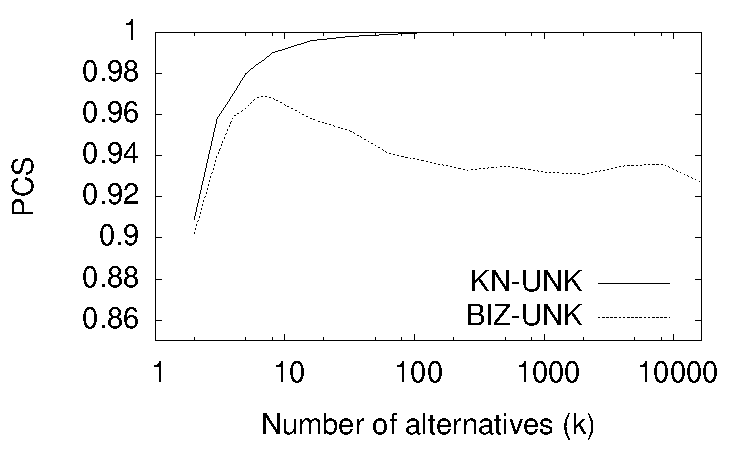
\includegraphics[width=2.9in]{pdf/FINAL-UNK-MDMINCA-PCS}
    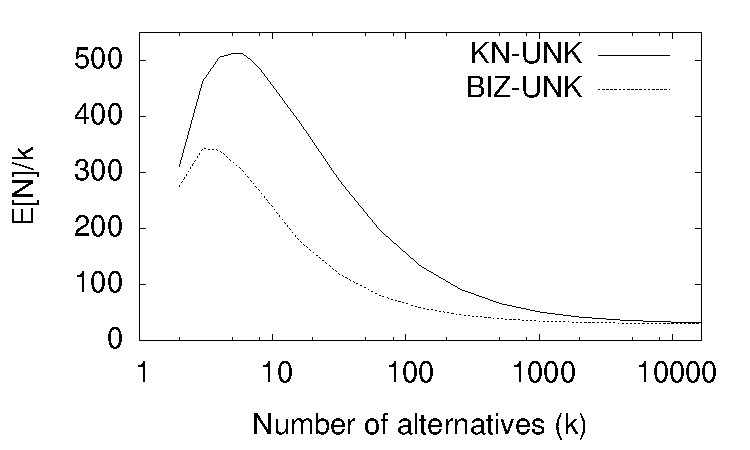
\includegraphics[width=2.9in]{pdf/FINAL-UNK-MDMDECA-Nk} 
    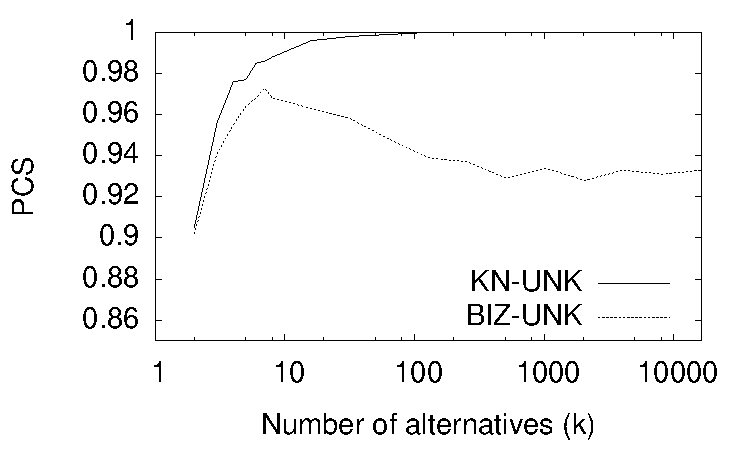
\includegraphics[width=2.9in]{pdf/FINAL-UNK-MDMDECA-PCS}
    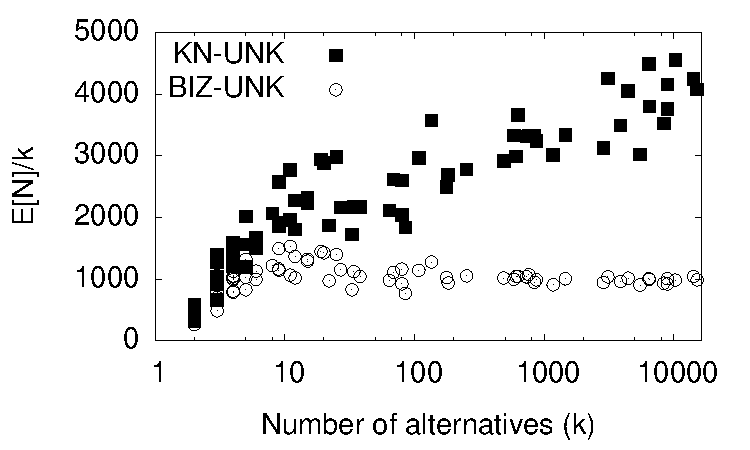
\includegraphics[width=2.9in]{pdf/FINAL-UNK-RPIHETA-Nk} 
    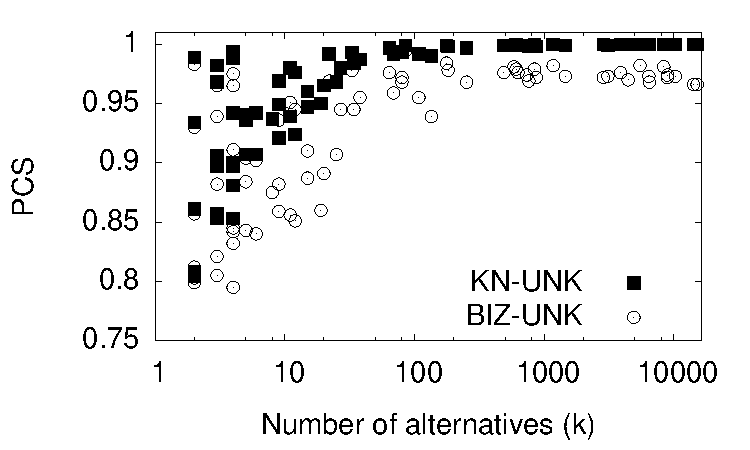
\includegraphics[width=2.9in]{pdf/FINAL-UNK-RPIHETA-PCS}

    \caption{Heterogeneous unknown variance, factor of 2 between largest and smallest variances.
    Row 1: SCINC;
    Row 2: SCDEC;
    Row 3: MDMINC;
    Row 4: MDMDEC;
    Row 5: RPIHET.
    }
  \end{figure}

  \begin{figure}[tb]
    \center
    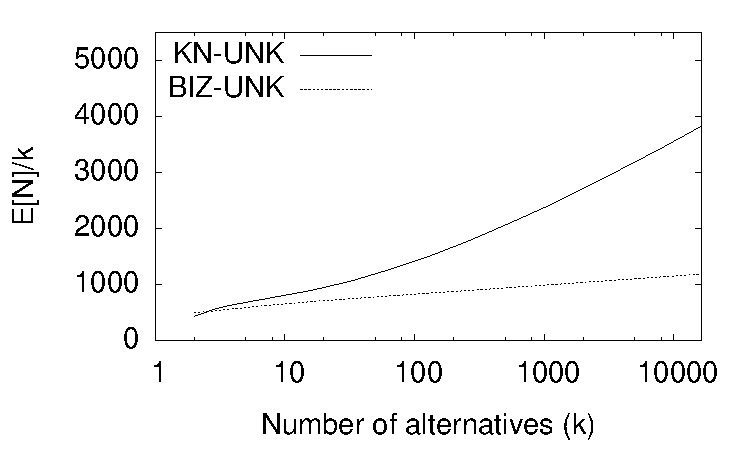
\includegraphics[width=2.9in]{pdf/FINAL-UNK-SCINC-Nk} 
    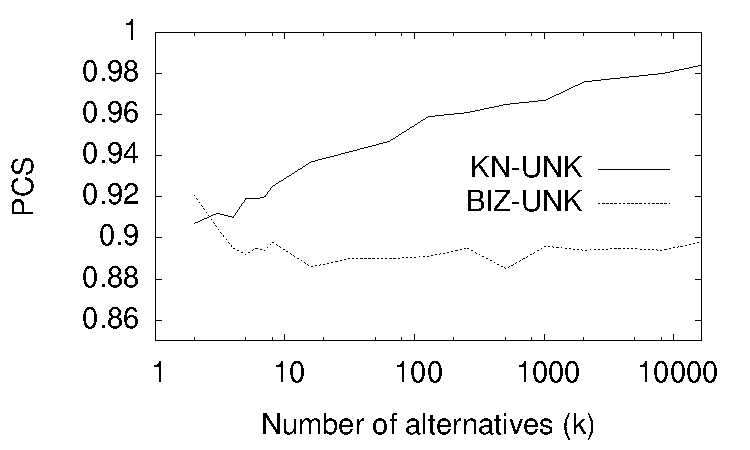
\includegraphics[width=2.9in]{pdf/FINAL-UNK-SCINC-PCS}
    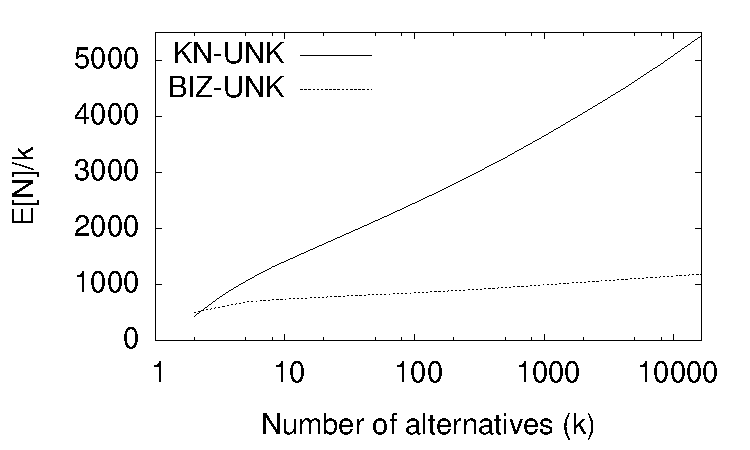
\includegraphics[width=2.9in]{pdf/FINAL-UNK-SCDEC-Nk} 
    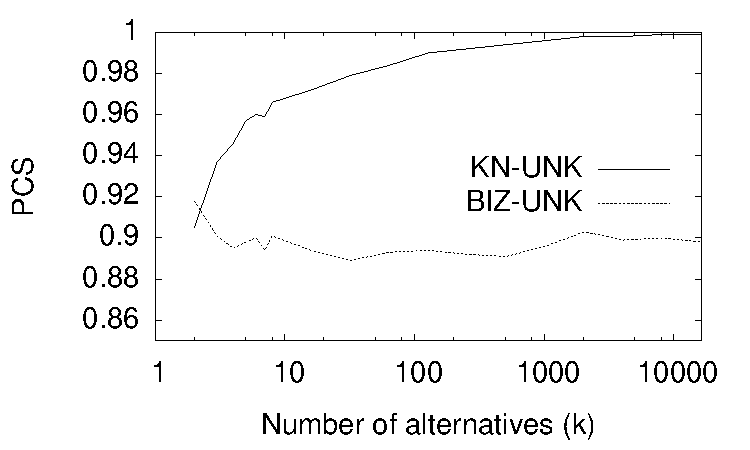
\includegraphics[width=2.9in]{pdf/FINAL-UNK-SCDEC-PCS}
    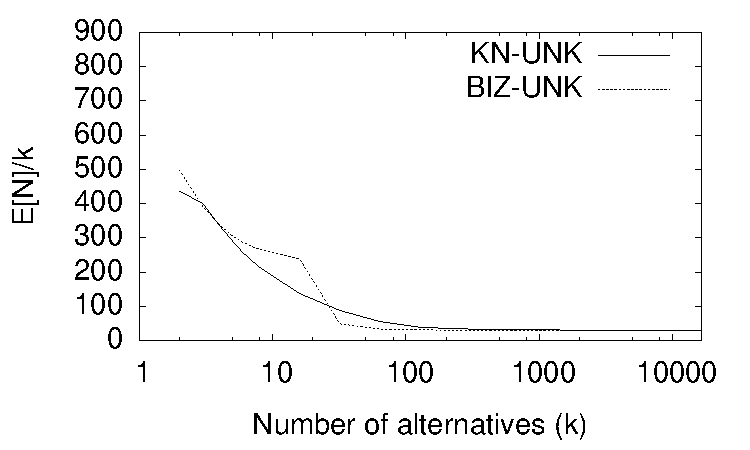
\includegraphics[width=2.9in]{pdf/FINAL-UNK-MDMINC-Nk} 
    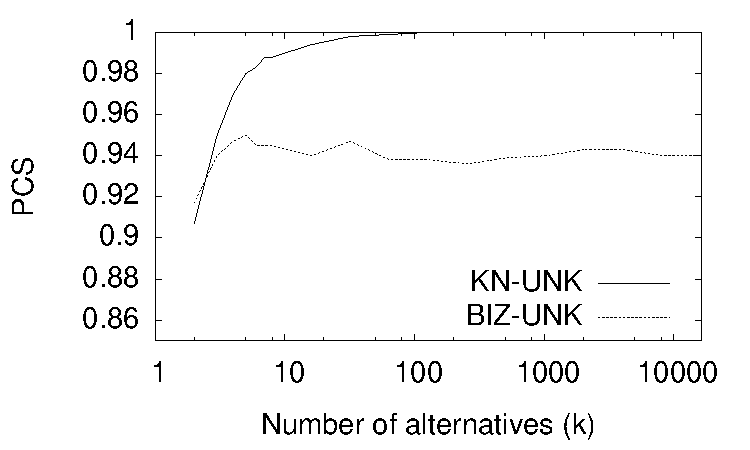
\includegraphics[width=2.9in]{pdf/FINAL-UNK-MDMINC-PCS}
    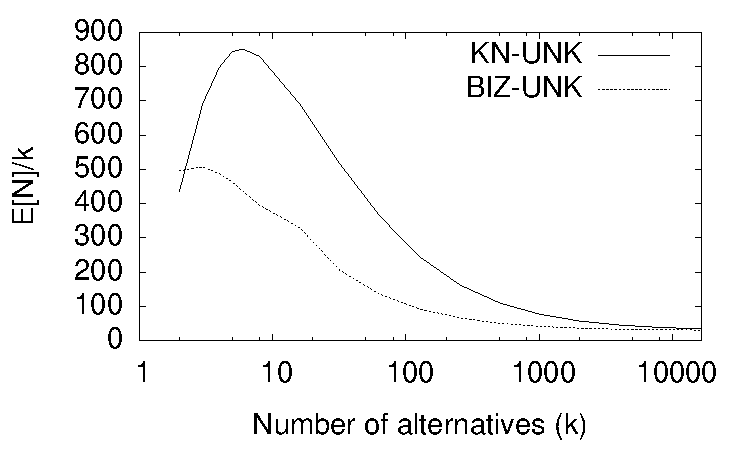
\includegraphics[width=2.9in]{pdf/FINAL-UNK-MDMDEC-Nk} 
    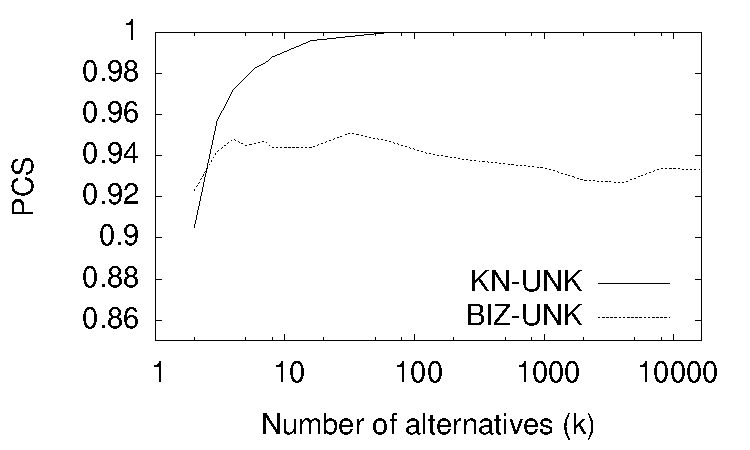
\includegraphics[width=2.9in]{pdf/FINAL-UNK-MDMDEC-PCS}
    \includegraphics[width=2.9in]{pdf/FINAL-UNK-RPIHET-Nk} 
    \includegraphics[width=2.9in]{pdf/FINAL-UNK-RPIHET-PCS}

    \caption{Heterogeneous unknown variance, factor of 16 between largest and smallest variances.
    Row 1: SCINC;
    Row 2: SCDEC;
    Row 3: MDMINC;
    Row 4: MDMDEC;
    Row 5: RPIHET.
    }
  \end{figure}


% Improvement factors
\begin{figure}[tb]
    \center
    \includegraphics[width=2.9in]{pdf/FINAL-Common-Known-ImprovementFactor}
    \includegraphics[width=2.9in]{pdf/FINAL-Common-Unknown-ImprovementFactor}
    \includegraphics[width=2.9in]{pdf/FINAL-HeteroA-Known-ImprovementFactor}
    \includegraphics[width=2.9in]{pdf/FINAL-Hetero-Known-ImprovementFactor}
    \includegraphics[width=2.9in]{pdf/FINAL-HeteroA-Unknown-ImprovementFactor}
    \includegraphics[width=2.9in]{pdf/FINAL-Hetero-Unknown-ImprovementFactor}

    \caption{Improvement factors.  
    (Top left) Common known variance.  
    (Top right) Common unknown variance.  
    (Middle left) Heterogeneous known variance, factor of 2 between largest and smallest variance.
    (Middle right) Heterogeneous known variance, factor of 16 between largest and smallest variance.
    (Bottom left) Heterogeneous unknown variance, factor of 2 between largest and smallest variance.
    (Bottom right) Heterogeneous unknown variance, factor of 16 between largest and smallest variance.
  }
  \end{figure}

% PGS plot
\begin{figure}[tb]
    \center
    \includegraphics[width=4in]{pdf/FINAL-PGS}

    \caption{Probability of Good Selection under BIZ, as a function of the
    distance between the best and the second best alternatives, for different
  numbers of alternatives $k$.}
  \end{figure}



\end{document}
